
\subsubsection{10.10.14}

\begin{enumerate}
	\item The time of beginning and ending of the congregation:
	18:30 - 21:40
	\item Purposes of the congregation:
	\begin{enumerate}
	  \item Choose the optimal diameter of the cross beams to the lift.
	  
	  \item Cut the aluminum profile into segments of desired length, drill them in the desired holes and install them between the rails instead of the layer, that made with original tetrix details.
	  
    \end{enumerate}
	\item Work, that has been done:
	\begin{enumerate}
	  \item The belt for moving apart the lift was bought.
	  
	  \begin{figure}[H]
	  	\begin{minipage}[h]{0.2\linewidth}
	  		\center  
	  	\end{minipage}
	  	\begin{minipage}[h]{0.6\linewidth}
	  		\center{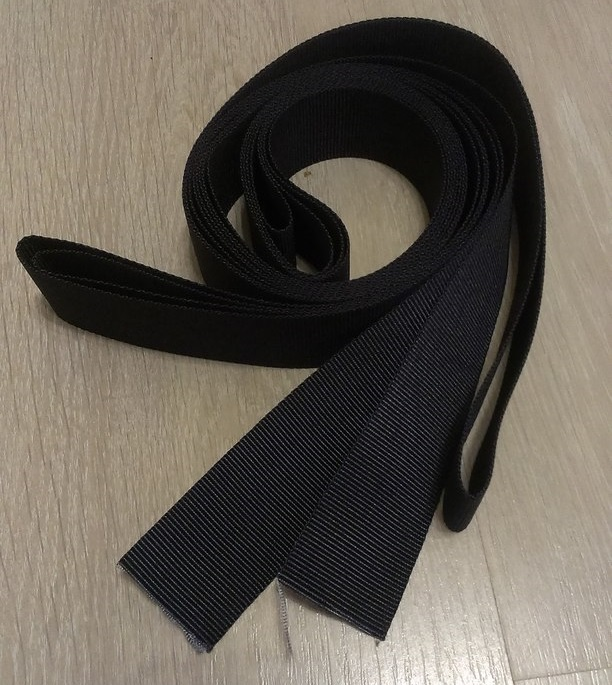
\includegraphics[scale=0.3]{days/10.10.14/images/01}}
	  		\caption{Belt}
	  	\end{minipage}
	  \end{figure}
      
      \item  To create bindings for cross beams was bought aluminum strip dimensions 200 cm x 5 cm x 0.2 cm.
      
      \item As the cross beams in the set are available TETRIX cylindrical rollers of 15 mm diameter and axis diameter of 5 mm. Preference was given to axes because of the compactness of the axes.
       
      \item Since the axis of the smaller diameter were cut edge to secure the wheel hubs, they resisted the movement of the belt. Then it was decided to impose on the axis free (without attachments) sleeve. Preliminary tests demonstrated the viability of the idea.
        
      \item After that, it was decided to take action:
      \begin{enumerate}
      	\item The guide lift were previously disassembled.
      	
      	\item  Aluminum strip was cut into 6 portions: 2 to 30 cm and 4 to 35 cm.
      	
      	\item When we were drilling details, some troubles appeared, because all drills were ground off. By the next session, it was decided to buy a new drill.
      	
      	\begin{figure}[H]
      		\begin{minipage}[h]{0.2\linewidth}
      			\center  
      		\end{minipage}
      		\begin{minipage}[h]{0.6\linewidth}
      			\center{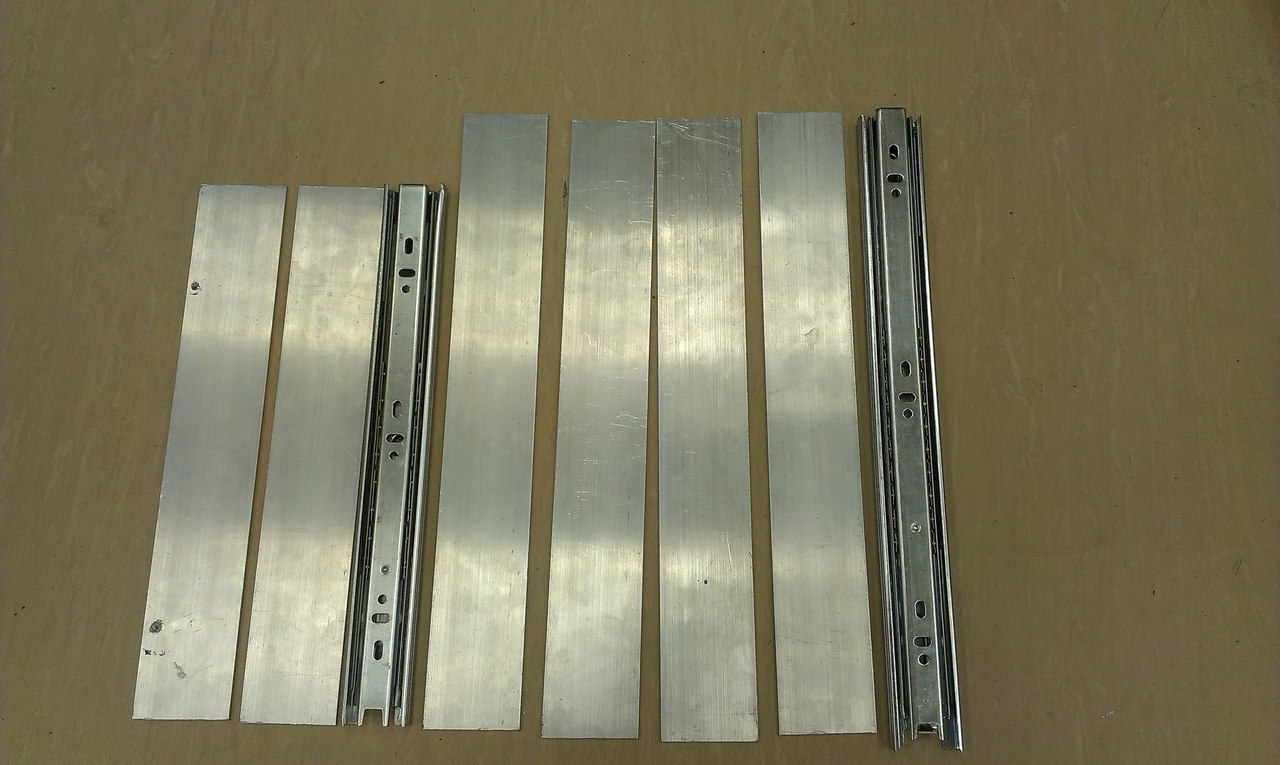
\includegraphics[scale=0.2]{days/10.10.14/images/02}}
      			\caption{Aluminum strip was cut into 6 portions}
      		\end{minipage}
      	\end{figure}
      	
      \end{enumerate}
      
    \end{enumerate}
    
	\item Results:
	\begin{enumerate}
	  \item Tracks for the lift was choosen.
	  
	  \item Beam have sawed into segments of desired length.
	  
	  \item Drill holes failed.
	   
    \end{enumerate}
    
	\item Tasks for the next congregations:
	\begin{enumerate}
	  \item Buy new drill for metal.
	  
    \end{enumerate}     
\end{enumerate}
\fillpage
